\documentclass{sig-alternate}

\usepackage{color}

\begin{document}
\conferenceinfo{OZCHI}{'14, Dec 2-5, 2014, Sydney, Australia}

\title{Visualising a Live Coding Arts Process {\color{red}[Draft]}}

\numberofauthors{3} 
\author{
\alignauthor Arrian Purcell\\
       \affaddr{Australian National University}\\
       \affaddr{Canberra, Australia}\\
       \email{u5015666@anu.edu.au}
\alignauthor Henry Gardner\\
       \affaddr{Australian National University}\\
       \affaddr{Canberra, Australia}\\
       \email{henry.gardner@anu.edu.au}
\alignauthor Ben Swift\\
       \affaddr{Australian National University}\\
       \affaddr{Canberra, Australia}\\
       \email{ben.swift@anu.edu.au}
}

\maketitle
\begin{abstract}

%Past software visualisations have typically focussed on visualising the software structures, the runtime behaviour or the source code. Within these categories, the process involved in developing the software is often overlooked. 

We have considered software visualisations as a means of communicating the real-time programming process of a ``livecoding" computer-music performance. Following a field study at a festival of the contemporary arts, two sets of complementary, interaction-driven visualisations were developed and incorporated into a livecoding system. A formal audience experiment was then undertaken to compare these visualisations and to survey their contributions to the audience experience, with emphasis on the two axes of ``understanding" and ``enjoyment" . The reactions of the  livecoding performer (the programmer) were also evaluated in a process of video-cued recall. 

%One field study and one controlled laboratory experiment were conducted in order to examine the effectiveness of visusalisations in communicating the software development process and communicating the programmer's intention. The field study investigated existing mental models of a programmer and an audience within the live coding context informing the mapping of software development process concepts to visual elements. The controlled laboratory experiment examined the effectiveness in aligning the audience's mental model with that of the programmer.

%The effectiveness of the visualisations developed is demonstrated in communicating the software development process and potential is shown for visualisations to further communicate the programmer's intention. The ongoing challenge is to match the audience's mental model with that of the programmer to further align the audience's understanding with that of the programmer.

The visualisations in the audience/user experiment appeared to positively contribute to the enjoyment of the audience. Although the results also demonstrated a the potential for visualisation to communicate the livecoding performer's intention to an audience their impact on ``understanding" did not seem to be sustained for the duration of a performance as well as they might. In addition, there remains an ongoing challenge to match the audience's mental model with that of the programmer.

\end{abstract}

\category{H.5}{Information Interfaces and Presentation}{Miscellaneous}

% \terms{Theory}

\keywords{live coding, software visualisation}

\section{Introduction}


``Show us your screens ... Code should be seen as well as heard'', says the draft manifesto of the international organisation ``TopLap'' [ref: http://toplap.org/wiki/ManifestoDraft] which is devoted to the decade-old arts performance practice ``livecoding''. Livecoding is a performance practice where computer code is created in front of a live audience to generate computer music, video and visualisations in real time. The ``show us your screens'' exhortation underscores the need for authenticity to distinguish this artform from aligned performance art genres such as VJ'ing. Live computer music is the primary product of livecoding. Where they exist, livecoding graphics and video are launched and orchestrated directly by commands from the computer keyboard for artistic impact. Commonly, non-expert livecoding audience members spend much of their time staring at raw computer code (text-based or visual programming languages) and, until now, no formal study has ever been undertaken to gauge an audience's understanding of that computer code and whether, from an audience perspective, code really should be ``seen as well as heard''. 

In this paper, we set out to evaluate the audience reception to the display of code during livecoding performances and to see whether code-driven visualisations  might improve both the audience enjoyment the audience understanding of the process of a livecoding performance.
  
Many traditional approaches to visualising code focus on the structure, behaviour or representation of software rather than the {\it process of programming} (e.g. the foundational references of \cite{Ball1996} and \cite{Price1992}) (ARE THEY FOUNDATIONAL? IF NOT WHY CITE THESE OLD THINGS? FIND THE FOUNDATIONAL ONES AND CITE THEM.) Until the present time, the academic treatment of visualisations of artistic livecoding have adopted a design or survey approach (ref: McLean et all, 2010, and perhaps other references) and have not subjected alternatives to rigorous evaluation.



{\color{red}[discuss literature]}

{\color{red}[discuss reason behind these studies]}

\section{Field Study}

%A field study was conducted to investigate the existing audience live coding mental model of the programming process. An audience was surveyed following a live coding performance regarding their understanding and enjoyment throughout the performance.

On one evening of the (name withheld for blind reviewing) arts festival in (withheld), 
a survey was presented to the audience of a livecoding computer-music performance. The survey was designed to gain an impression of the audience response to the performance and to the projection of the computer code (a Scheme type of language with syntax highlighting). Alongside demographic and open-ended questions, audience members were solicited to indicate which of a number of curves best represented their personal ``enjoyment" and ``understanding" of the performer's actions in typing the computer code through the performance. These curves were analysed based on their binning into ``high", ``medium", and ``low'' categories for the ``beginning'', ``middle'' and ``end'' of the performance. Other survey questions addressed the sense of ``liveness'' of the performance and whether the code-projections were found to be confusing. 

%A total of thirteen survey responses were received and a small number of audience members, known to the researcher, were selected for a follow-up interview. 

%\subsection{Results}

%A total of thirteen survey responses were received. Of these, $77\%$ regularly listen to music and $54\%$ perform regularly. $38\%$ of the respondents have high exposure to programming through work, study or their hobbies, as opposed to $31\%$ who have no experience with it. 

Of the 13 survey respondences received, 6 indicated a high level of enjoyment throughout the whole performance with the remaining 7 responses mostly indicating alternating levels of enjoyment. No responses indicated a low level of enjoyment throughout the performance.

%The results suggest an overall high level of enjoyment of the performance. No respondents chose low enjoyment throughout the performance.

%Similarly, understanding was measured according to the relative change in understanding through the performance from the beginning to the end. 

%$31\%$ of survey respondents had no change to understanding through the performance. 

Only 2 of the 13 respondents indicated that they understood the relationship between the code projections and the music throughout the performance. Although a Chi-square analysis revealed no statistical significance between ``enjoyment'' and ``understanding'' per se, it was remarkable the that 3 of the 6 respondents who indicated a high level of enjoyment throughout the performance, also indicated a pattern of their understanding increasing from low to high as the performance progressed. Nine of the 13 respondents stated that the code projections provided a sense of liveness to the performance and the remainder stated that these visuals had no effect on their sense of liveness. Four respondents felt that the code projections were confusing, 5 stated that they were not, and 4 did not answer the question. 

%Overall, understanding is spread out more than enjoyment with only $15\%$ suggesting that they could understand the relationship between the visuals and the music throughout the performance. 

%There is no statistically significant relationship ($p > .05$) between music listening habits and understanding nor is there a statistically significant relationship ($p > .05$) between coding experience and understanding.

%Notably, within the relationship between enjoyment and understanding, three respondents who had high enjoyment throughout the performance were the only respondents who had a pattern of low to high understanding. However, the relationship between enjoyment and understanding is not statistically significant ($p > .05$).

%$69\%$ of respondents stated that the visuals provided a sense of liveness to the performance. The remained $31\%$ stated that they had no effect on their sense of liveness. There were no responses stating that the visuals negatively impacted the sense of liveness.
%In terms of confusion, $38\%$ suggested that no aspects of the visuals were confusing, though $31\%$ did not respond to the question.

%\subsection{Discussion}

{\color{red}[split results into results + discussion]}



NO REAL NEED TO SAY MUCH HERE. ELIMINATE THE SUBSECTION HEADING. SUBSECTIONS TAKE UP SPACE.

Taken as a whole, the results of this small field study were somewhat salutory for the notion of ``seeing as well as hearing" code during a livecoding performance, especially as far as the general public is concerned. The best that can be said for the code projections is that a majority of the audience felt that they made the performance seem more ``live". However a minority stated that they found the projections confusing and only a very small number of respondents claimed to have actually understood what the programmer was doing. We were quite intrigued by the small cohort of respondents whose understanding increased through the performance and whose ejoyment remained high, and we wished to test whether augmenting code projections with additional visualistions might increase this pattern of understanding, and enjoyment across an audience. 

\section{Design}

Two sets of visualisations were developed based on the results of the initial survey and the literature. The first set focussed on increasing audience retention and interest through maximising aesthetic appeal. The second set attempted to communicate and highlight the actions of the programmer. These two approaches will be referred to as the `aesthetic' condition and the `didactic' condition respectively.

The aesthetic visualisations mapped the ...

The didactic visualisations mapped the ...

{\color{red}[discuss design considerations, mappings and justify in the literature]}

{\color{red}[representative images of the visualisations]}

The set of didactic visualisations predominantly focussed on the relationship between the live coding active processes and their behaviour. The visualisations prominently displaying the names of the active functions with visual indication of the number of functions running and their callback time. Bright colours and solid shapes were used to ensure constant visibility and communicate the intention of the underlying code. Overall, four visualisations were presented with each introduced depending on the number of active functions. It was predicted that taking a more educational approach would see a reduction in audience confusion through the performance.

The set of aesthetic visualisations focussed less on the programmatic aspects of the live coding performance, rather intending to provide additional visual interest to the projected code thereby prolonging attention. More variety was used in visual structure and colour. Again, four visualisations were presented, varying the visualisation based on the number of active functions. It was predicted that focussing on the aesthetic nature of the visualisations would assist in audience retention and result in a consistency of interest through the performance.

\section{User Study}

%The two sets of visualisations developed were examined in a live coding context to determine effective presentational and educational features. The goal of this study was to determine the usability, differences and desirability of the two approaches to further inform future live coding visualisations.

Explain the nuts and bolts of the user study here. 

\subsection{Results}

Understanding and enjoyment were evaluated against the didactic and aesthetic visualisations. Results and statistical analysis of the differences between the aesthetic and didactic conditions follows. Note that for the following statistical analysis a significance level of $0.05$ was used with the chi-squared test for independence.

HOW MANY RESPONSES? ETC. YOU MUST DESCRIBE YOUR EXPERIMENT AND THE ANALYSIS THAT YOU CARRIED OUT.

\subsubsection{Understanding}

THIS AND SUBSEQUENT SECTIONS ARE A BIT LABORIOUS. CUT THEM DOWN AND DO AWAY WITH SUBSECTION HEADINGS

Overall, $37\%$ participants stated specifically that the didactic visualisations helped them to understand the code, whereas $12\%$ participants stated that the aesthetic visualisations assisted in understanding the code. A significant difference between the visualisations effect on understanding was found ($\chi^2=7.1986,df=2,p=0.02734$).

\subsubsection{Enjoyment}
Overall, for both visualisations, a large proportion ($> 50\%$) of the participants stated that the visualisations helped their enjoyment of the performance. Of the participants, $76\%$ stated that the aesthetic visualisations helped their enjoyment compared to $56\%$ participants that stated the didactic visualisations helped their enjoyment. No significant difference between the two visualisations effect on enjoyment was found ($\chi^2=3.7733,df=2,p=0.1516$).

\subsubsection{Change in Understanding}

\begin{figure}
\centering
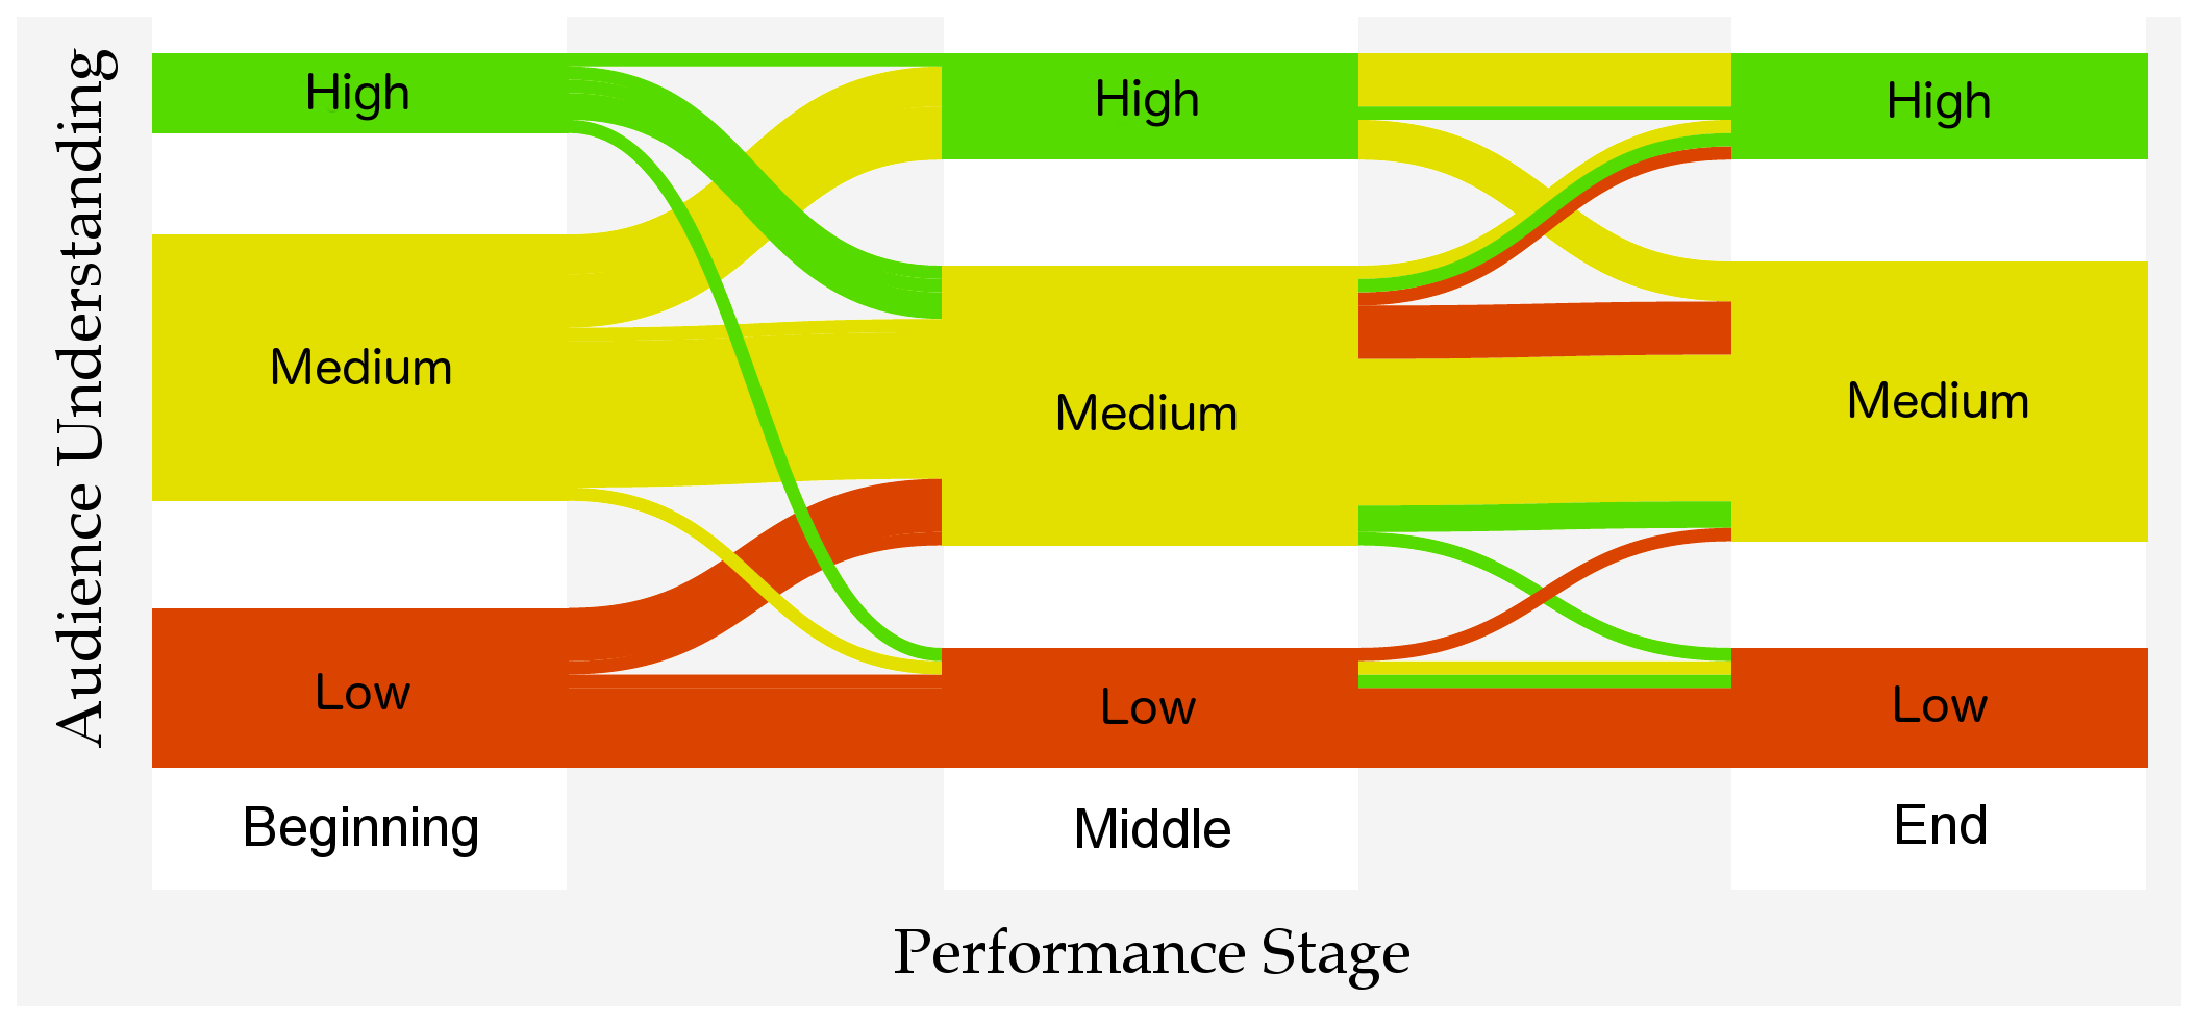
\epsfig{file=aesthetic-understanding-final.eps, width=3.4in}
\caption{Audience understanding during the performances with the aesthetic condition.}
\end{figure}

\begin{figure}
\centering
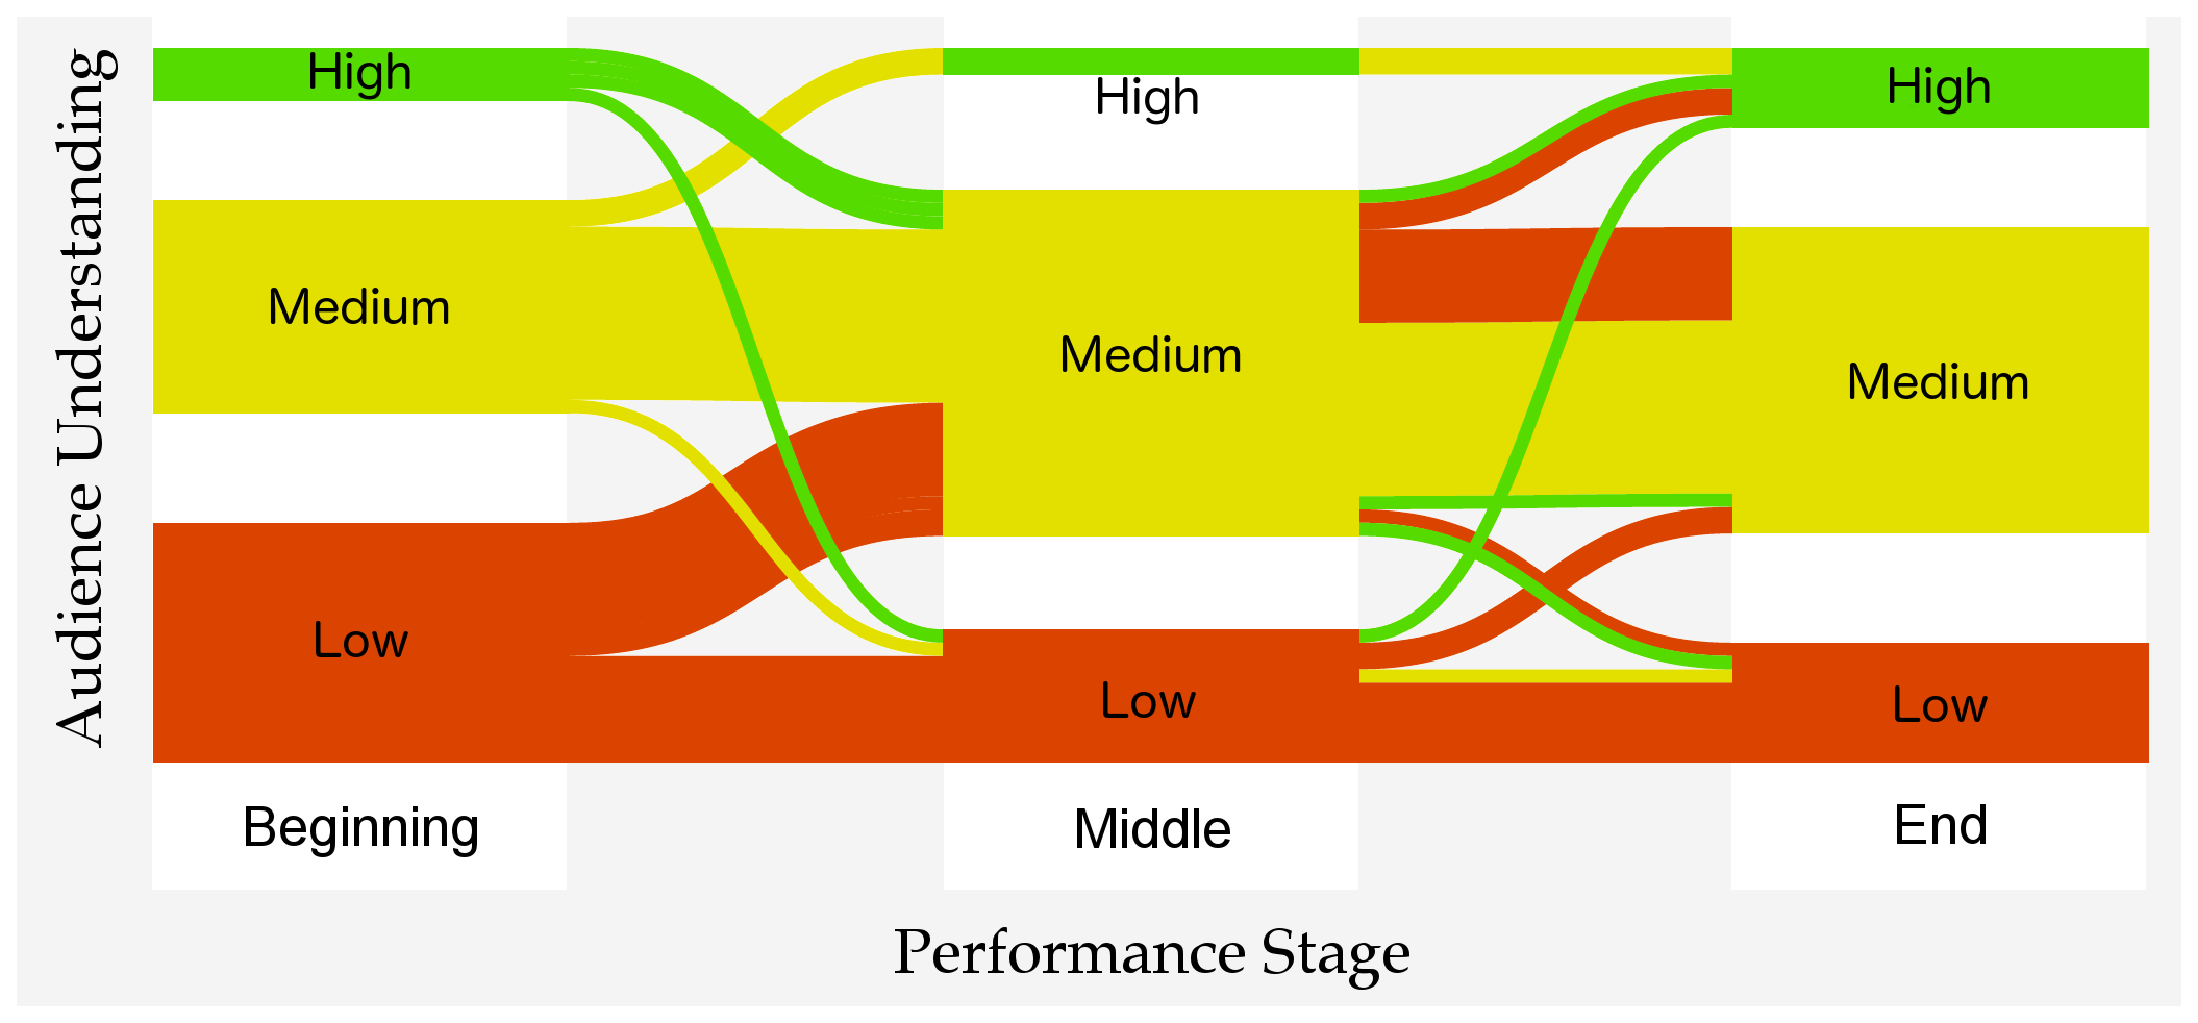
\epsfig{file=didactic-understanding-final.eps, width=3.4in}
\caption{Audience understanding during the performances with the didactic condition.}
\end{figure}

Participants were asked to rate their understanding during the beginning, middle and end of the performance.

During the didactic and aesthetic performances, $49\%$ and $44\%$ of the participants respectively stated that their understanding remained the same throughout the performance.

During the didactic performance, $10\%$ of the audience had an understanding that tended downwards (eg. high to low) compared to $20\%$ of the audience during the aesthetic performance meaning fewer audience members had a reduction in understanding through the didactic performance.

\subsubsection{Change in Enjoyment}

\begin{figure}
\centering
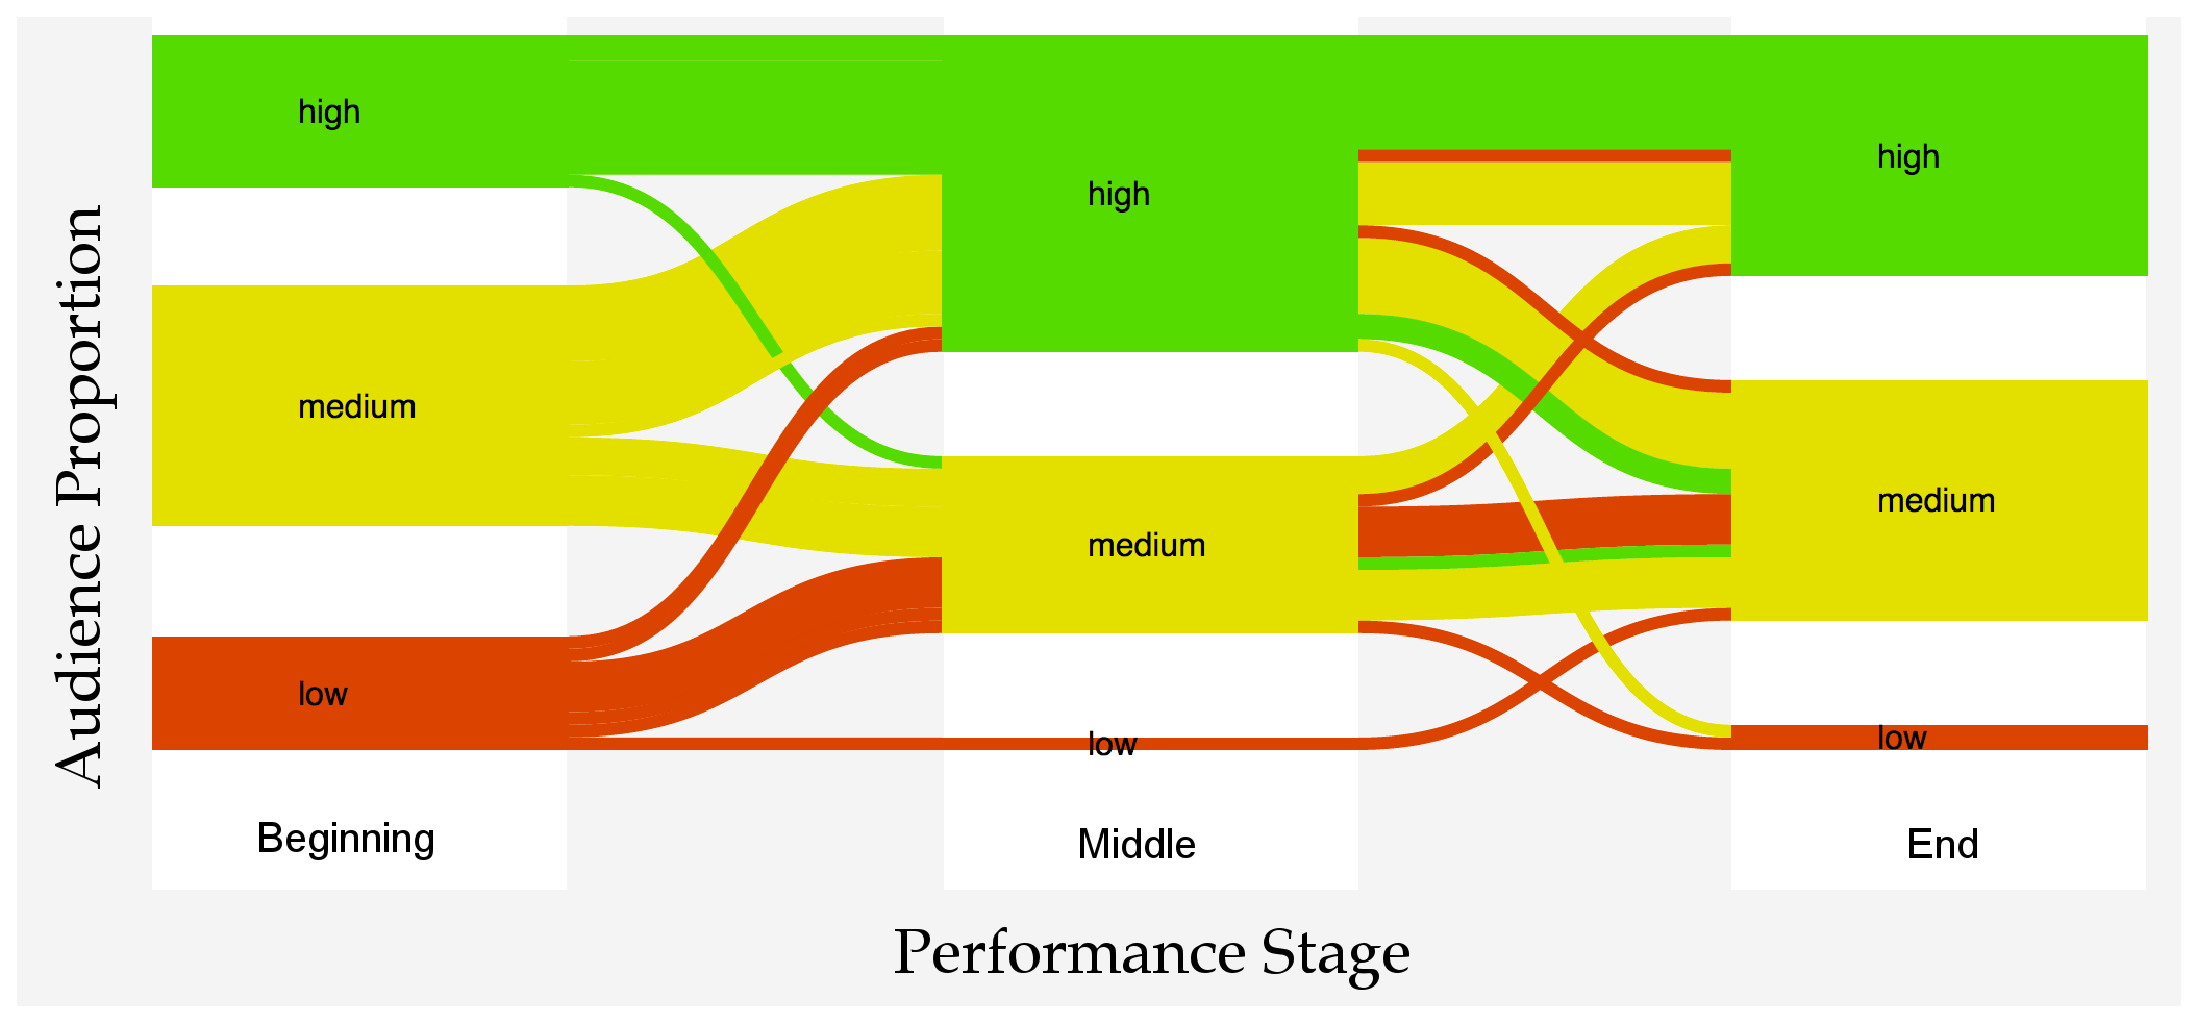
\epsfig{file=aesthetic-enjoyment-final.eps, width=3.4in}
\caption{Audience enjoyment during the performances with the aesthetic condition.}
\end{figure}

\begin{figure}
\centering
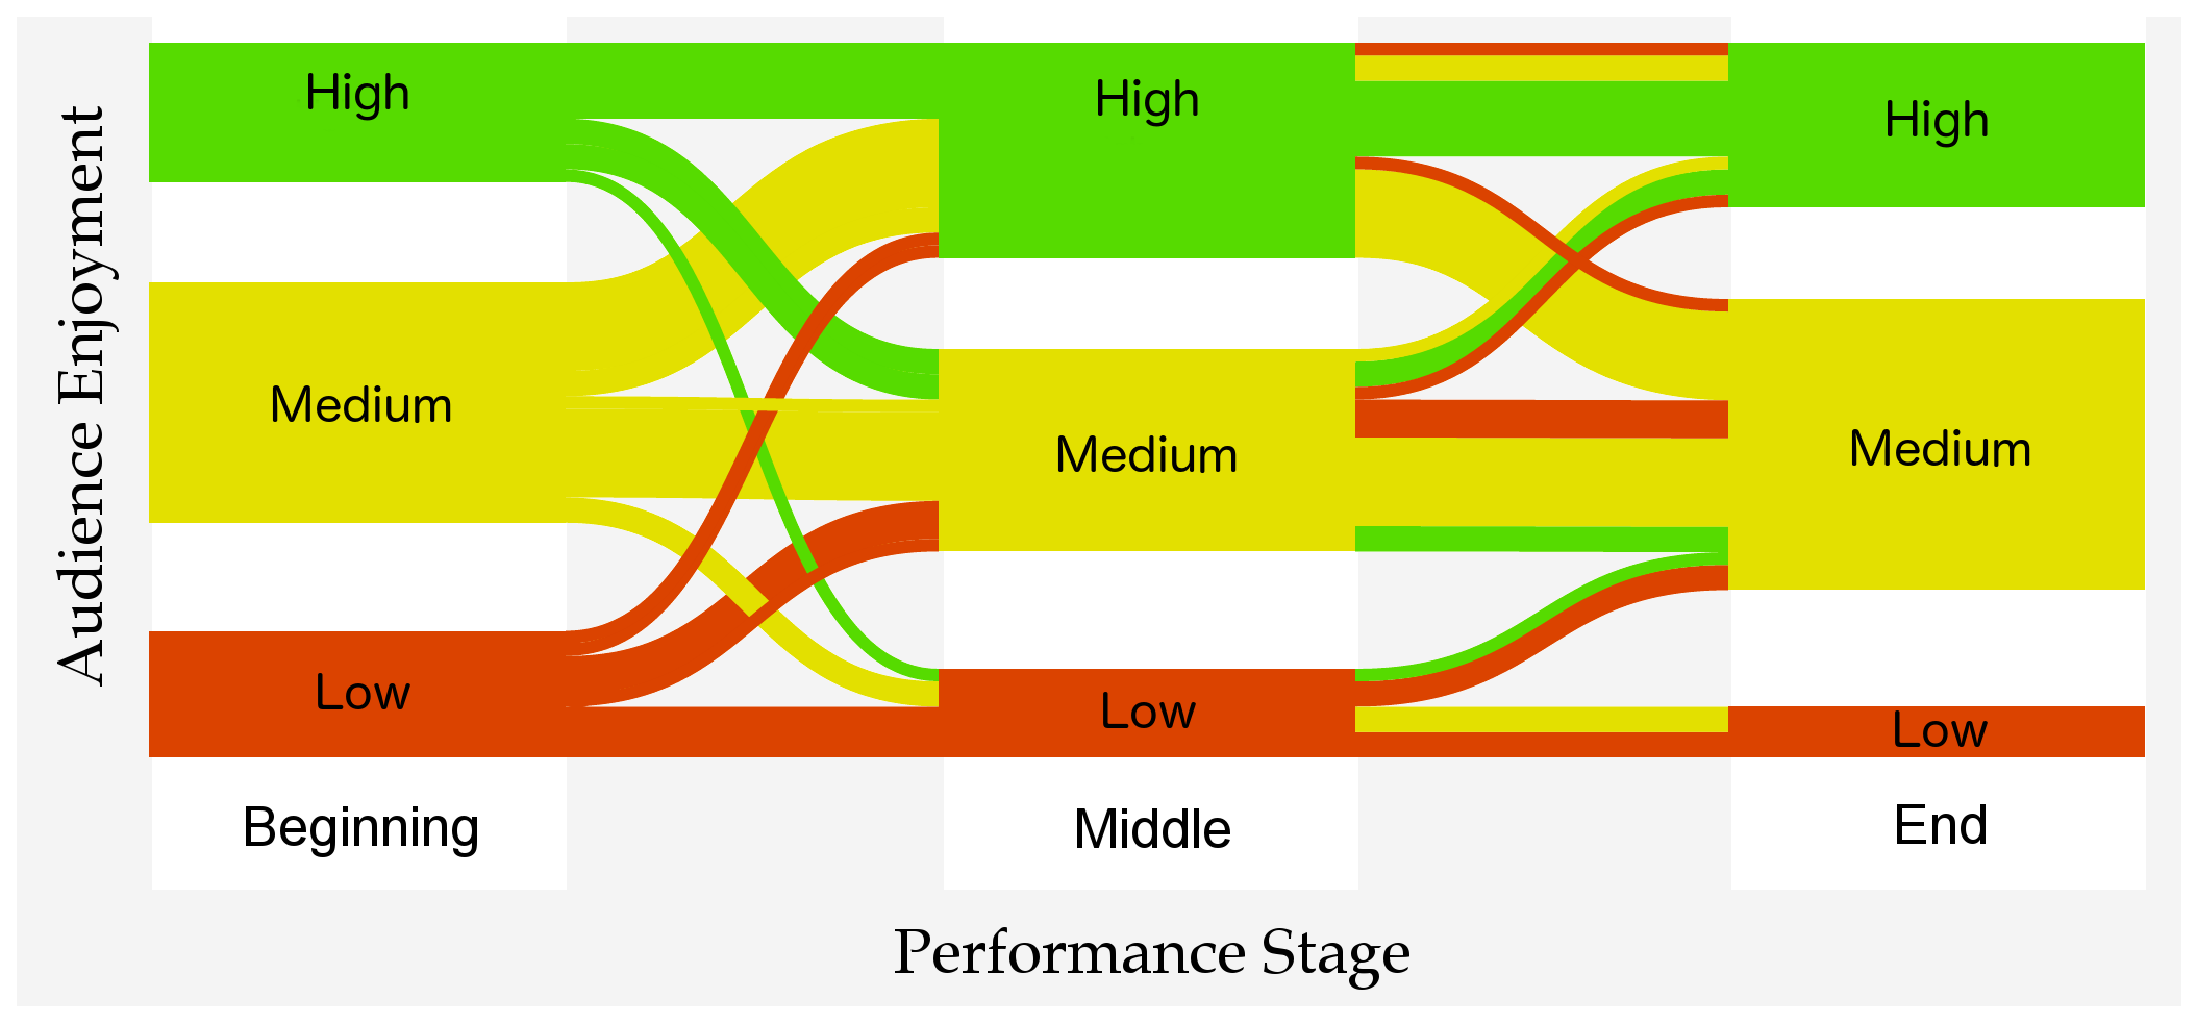
\epsfig{file=didactic-enjoyment-final.eps, width=3.4in}
\caption{Audience enjoyment during the performances with the didactic condition.}
\end{figure}

Participants were asked to rate their enjoyment during the beginning middle and end of the performance.

During the didactic performance, $15\%$ of the audience stated that enjoyment increased during the beginning remaining steady for the remainder whereas $24\%$ of the audience said the same during the aesthetic performance.

During the didactic performance, $22\%$ of the audience stated that their enjoyment decreased during the start of the performance whereas only $2\%$ stated the same for the aesthetic performance.

Approximately $30\%$ of the audience during both the aesthetic and didactic performances stated that their enjoyment remained steady throughout.

\subsubsection{Liveness}

Participants were asked to discuss how each visualisation influenced or impacted the liveness of the performance. Concepts identified included positive and negative valence towards the didactic visualisations, positive and negative valence towards the aesthetic visualisations and the relevance of visual source code. 

within the discussion included the positive and negative aspects of the didactic visualisations, the positive and negative aspects of the aesthetic visualisations, source code discussion and statements indicating an understanding between the visuals and the source code.

Overall, $54\%$ of the audience indicated negative valence towards the didactic visualisation regarding liveness referencing a variety of reasons including that the ``visuals only responded to what was typed'', that the ``musical forms didn't occur at the most expected times'' and that the visualisations ``perhaps made the performance seem too polished''.

On the other hand, $34\%$ of the audience indicated positive valence towards the didactic visualisations suggesting that ``it was easier to follow this visualisation than the code'', ``the visualisations clearly showed the changes being made to the code'' and that these visualisations ``helped more with communicating that the performance was live''.

$40\%$ of the audience had negative valence towards the aesthetic visualisation its effect on the sense of liveness. Reasons cited include that the ``influence is not clear'' between the code and the visuals, that ``the visualisation did not make much sense'' and that the ``visualisations did nothing to suggest that the performance was live''.

$32\%$ had positive valence towards the aesthetic visualisation. A variety of the response included that these visuals were ``less dominating and more complementary'' and that ``the visualisations helped to show when a piece of code started working''.

A relatively large proportion ($28\%$) of the audience discussed the importance of the source code to the sense of liveness of the performance such as that the ``code showed what the musician was doing physically''. A further $5\%$ of the audience demonstrated a deeper understanding of the live coding process such as ``changing values produced changes in tone and speed of the music pitch''.

\subsection{Discussion}

THIS SECTION IS BETTER. IT COMMUNICATES THE MAIN MESSAGES. STILL IT COULD BE EDITED DOWN.

Overall enjoyment of the visualisations was high. This was the case for both the aesthetic and didactic visualisations.

The enjoyment of the aesthetic visualisation was higher and generally increased during the earlier stages of the performances suggesting that the aesthetic visualisations held the audience's attention consistently for a longer period.

The didactic visualisation had a more constant decrease in enjoyment throughout the performance. Audience suggested improvements offer some insight with some stating that the visualisations were competing with the projected code. One audience member stated that they ``found them distracting'' and that they ``preferred just to read the code''. Given that more than half of the audience stated that both visualisations contributed positively to enjoyment, there is indication that the didactic visualisations contributed more to audience fatigue through the performance with decreased effectiveness during the later stages of the performances.

As expected, the didactic visualisations had a clear educational benefit over the aesthetic visualisations, contributing to increased understanding throughout the performance. Nevertheless, features of the visualisation still confused the audience. For example, one audience member stated that ``it felt harder to understand the code'' during the didactic performance than the aesthetic performance. Similarly, a number of audience members discussed the need for a better relationship between the visualisation and the music.

There was indication that the experience of the live coder and the experience of the audience was fundamentally different. For example, many members of the audience stated that they drifted between focussing on the music, focussing on the visualisations and focussing on the code. However, the live coder stated in the interview that his focus was dedicated purely to the code and the music rarely drifting. In one particular section of the interview, the live coder stated: ``I definitely wasn't paying attention to them on the day. In fact I tuned them out as best I can because I am just trying to focus on the code''. This conflicted with some members of the audience. For example, one stated that ``you could see the code being written and the visualisations helped to show when a piece of code started working''. 

The strategy for audience members for either understanding or enjoying the performance proved to be different to that of the live coder. Regarding distractions, one audience member stated that ``the visualisations were interesting but distracting''. In comparison, when asked if the visualisations were distracting the live coder stated: ``Ah, no. In general I'm just so focussed on the code''. This difference may be due to the varying experience levels or the pressure of the situation.

\section{Conclusions}

In the first systematic studies of their type, we have identified an opportunity for real-time code visualistations to improve the audience experience in a livecoding computer-music performance. With few exceptions, our survey of a livecoding performance revealed a generally low to medium level of audience understanding throughout that performance. Although almost half the survey respondents indicated a high level of enjoyment throughout, and more than half indicated a high level of appreciation of the ``liveness'' of that performance, 

 but a high level of appreciation of liveness and a high level of enjoyment. 

 Our comparison of two prototype code visulisations has indicated that some sort of ``understanding'' seems to result when an audience is subjected to a ``didactic'' code visualisation. 


An application of the visualisation of code to live coding has been examined. Results indicate the importance of providing visuals that complement the live coding performance. Visualisations targeted at the education of the audience showed an increase in understanding throughout the performance whereas visualisations targeted at the aesthetics of the music and performance indicated audience retention and a reduced fatigue effect over the didactic visualisations.

There was indication throughout audience feedback and the follow-up interview that the visualisations had potential. Desirable features within both visualisations could be further utilised building on the ideas developed including reacting instantly to code changes within the visualisations and providing a more effective visualisation of the relationship of code to music. These developments will provide a baseline for future visualisations.

Marshall McLuhan stated that ``
The business of art is no longer the communication of thoughts or feelings which are to be conceptually ordered, but a direct participation in an experience. The whole tendency of modern communication...is towards participation in a process, rather than apprehension of concepts." (ref: Letter to Harold Adam Innis, March 14 1951. From Essential McLuhan (1995), edited by Eric McLuhan and Frank Zingrone, p. 73)

Our hope is that future development of the research described in this paper will bring audiences into the process of livecoding in such a way that they can feel as though they are active (albeit virtual) collaborators of a highly skilled artist.

{\color{red}[summary + future work]}

% The \textit{proceedings} are the records of a conference.
% ACM seeks to give these conference by-products a uniform,
% high-quality appearance.  To do this, ACM has some rigid
% requirements for the format of the proceedings documents: there
% is a specified format (balanced  double columns), a specified
% set of fonts (Arial or Helvetica and Times Roman) in
% certain specified sizes (for instance, 9 point for body copy),
% a specified live area (18 $\times$ 23.5 cm [7" $\times$ 9.25"]) centered on
% the page, specified size of margins (1.9 cm [0.75"]) top, (2.54 cm [1"]) bottom
% and (1.9 cm [.75"]) left and right; specified column width
% (8.45 cm [3.33"]) and gutter size (.83 cm [.33"]).

% The good news is, with only a handful of manual
% settings\footnote{Two of these, the {\texttt{\char'134 numberofauthors}}
% and {\texttt{\char'134 alignauthor}} commands, you have
% already used; another, {\texttt{\char'134 balancecolumns}}, will
% be used in your very last run of \LaTeX\ to ensure
% balanced column heights on the last page.}, the \LaTeX\ document
% class file handles all of this for you.

% The remainder of this document is concerned with showing, in
% the context of an ``actual'' document, the \LaTeX\ commands
% specifically available for denoting the structure of a
% proceedings paper, rather than with giving rigorous descriptions
% or explanations of such commands.

% \section{The {\secit Body} of The Paper}
% Typically, the body of a paper is organized
% into a hierarchical structure, with numbered or unnumbered
% headings for sections, subsections, sub-subsections, and even
% smaller sections.  The command \texttt{{\char'134}section} that
% precedes this paragraph is part of such a
% hierarchy.\footnote{This is the second footnote.  It
% starts a series of three footnotes that add nothing
% informational, but just give an idea of how footnotes work
% and look. It is a wordy one, just so you see
% how a longish one plays out.} \LaTeX\ handles the numbering
% and placement of these headings for you, when you use
% the appropriate heading commands around the titles
% of the headings.  If you want a sub-subsection or
% smaller part to be unnumbered in your output, simply append an
% asterisk to the command name.  Examples of both
% numbered and unnumbered headings will appear throughout the
% balance of this sample document.

% Because the entire article is contained in
% the \textbf{document} environment, you can indicate the
% start of a new paragraph with a blank line in your
% input file; that is why this sentence forms a separate paragraph.

% \subsection{Type Changes and {\subsecit Special} Characters}
% We have already seen several typeface changes in this sample.  You
% can indicate italicized words or phrases in your text with
% the command \texttt{{\char'134}textit}; emboldening with the
% command \texttt{{\char'134}textbf}
% and typewriter-style (for instance, for computer code) with
% \texttt{{\char'134}texttt}.  But remember, you do not
% have to indicate typestyle changes when such changes are
% part of the \textit{structural} elements of your
% article; for instance, the heading of this subsection will
% be in a sans serif\footnote{A third footnote, here.
% Let's make this a rather short one to
% see how it looks.} typeface, but that is handled by the
% document class file. Take care with the use
% of\footnote{A fourth, and last, footnote.}
% the curly braces in typeface changes; they mark
% the beginning and end of
% the text that is to be in the different typeface.

% You can use whatever symbols, accented characters, or
% non-English characters you need anywhere in your document;
% you can find a complete list of what is
% available in the \textit{\LaTeX\
% User's Guide}\cite{Lamport:LaTeX}.

% \subsection{Math Equations}
% You may want to display math equations in three distinct styles:
% inline, numbered or non-numbered display.  Each of
% the three are discussed in the next sections.

% \subsubsection{Inline (In-text) Equations}
% A formula that appears in the running text is called an
% inline or in-text formula.  It is produced by the
% \textbf{math} environment, which can be
% invoked with the usual \texttt{{\char'134}begin. . .{\char'134}end}
% construction or with the short form \texttt{\$. . .\$}. You
% can use any of the symbols and structures,
% from $\alpha$ to $\omega$, available in
% \LaTeX\cite{Lamport:LaTeX}; this section will simply show a
% few examples of in-text equations in context. Notice how
% this equation: \begin{math}\lim_{n\rightarrow \infty}x=0\end{math},
% set here in in-line math style, looks slightly different when
% set in display style.  (See next section).

% \subsubsection{Display Equations}
% A numbered display equation -- one set off by vertical space
% from the text and centered horizontally -- is produced
% by the \textbf{equation} environment. An unnumbered display
% equation is produced by the \textbf{displaymath} environment.

% Again, in either environment, you can use any of the symbols
% and structures available in \LaTeX; this section will just
% give a couple of examples of display equations in context.
% First, consider the equation, shown as an inline equation above:
% \begin{equation}\lim_{n\rightarrow \infty}x=0\end{equation}
% Notice how it is formatted somewhat differently in
% the \textbf{displaymath}
% environment.  Now, we'll enter an unnumbered equation:
% \begin{displaymath}\sum_{i=0}^{\infty} x + 1\end{displaymath}
% and follow it with another numbered equation:
% \begin{equation}\sum_{i=0}^{\infty}x_i=\int_{0}^{\pi+2} f\end{equation}
% just to demonstrate \LaTeX's able handling of numbering.

% \subsection{Citations}
% Citations to articles \cite{bowman:reasoning,
% clark:pct, braams:babel, herlihy:methodology},
% conference proceedings \cite{clark:pct} or
% books \cite{salas:calculus, Lamport:LaTeX} listed
% in the Bibliography section of your
% article will occur throughout the text of your article.
% You should use BibTeX to automatically produce this bibliography;
% you simply need to insert one of several citation commands with
% a key of the item cited in the proper location in
% the \texttt{.tex} file \cite{Lamport:LaTeX}.
% The key is a short reference you invent to uniquely
% identify each work; in this sample document, the key is
% the first author's surname and a
% word from the title.  This identifying key is included
% with each item in the \texttt{.bib} file for your article.

% The details of the construction of the \texttt{.bib} file
% are beyond the scope of this sample document, but more
% information can be found in the \textit{Author's Guide},
% and exhaustive details in the \textit{\LaTeX\ User's
% Guide}\cite{Lamport:LaTeX}.

% This article shows only the plainest form
% of the citation command, using \texttt{{\char'134}cite}.
% This is what is stipulated in the SIGS style specifications.
% No other citation format is endorsed or supported.

% \subsection{Tables}
% Because tables cannot be split across pages, the best
% placement for them is typically the top of the page
% nearest their initial cite.  To
% ensure this proper ``floating'' placement of tables, use the
% environment \textbf{table} to enclose the table's contents and
% the table caption.  The contents of the table itself must go
% in the \textbf{tabular} environment, to
% be aligned properly in rows and columns, with the desired
% horizontal and vertical rules.  Again, detailed instructions
% on \textbf{tabular} material
% is found in the \textit{\LaTeX\ User's Guide}.

% Immediately following this sentence is the point at which
% Table 1 is included in the input file; compare the
% placement of the table here with the table in the printed
% dvi output of this document.

% \begin{table}
% \centering
% \caption{Frequency of Special Characters}
% \begin{tabular}{|c|c|l|} \hline
% Non-English or Math&Frequency&Comments\\ \hline
% \O & 1 in 1,000& For Swedish names\\ \hline
% $\pi$ & 1 in 5& Common in math\\ \hline
% \$ & 4 in 5 & Used in business\\ \hline
% $\Psi^2_1$ & 1 in 40,000& Unexplained usage\\
% \hline\end{tabular}
% \end{table}

% To set a wider table, which takes up the whole width of
% the page's live area, use the environment
% \textbf{table*} to enclose the table's contents and
% the table caption.  As with a single-column table, this wide
% table will ``float" to a location deemed more desirable.
% Immediately following this sentence is the point at which
% Table 2 is included in the input file; again, it is
% instructive to compare the placement of the
% table here with the table in the printed dvi
% output of this document.


% \begin{table*}
% \centering
% \caption{Some Typical Commands}
% \begin{tabular}{|c|c|l|} \hline
% Command&A Number&Comments\\ \hline
% \texttt{{\char'134}alignauthor} & 100& Author alignment\\ \hline
% \texttt{{\char'134}numberofauthors}& 200& Author enumeration\\ \hline
% \texttt{{\char'134}table}& 300 & For tables\\ \hline
% \texttt{{\char'134}table*}& 400& For wider tables\\ \hline\end{tabular}
% \end{table*}
% end the environment with {table*}, NOTE not {table}!

% \subsection{Figures}
% Like tables, figures cannot be split across pages; the
% best placement for them
% is typically the top or the bottom of the page nearest
% their initial cite.  To ensure this proper ``floating'' placement
% of figures, use the environment
% \textbf{figure} to enclose the figure and its caption.

% This sample document contains examples of \textbf{.eps}
% and \textbf{.ps} files to be displayable with \LaTeX.  More
% details on each of these is found in the \textit{Author's Guide}.

% \begin{figure}
% \centering
% 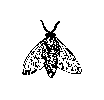
\epsfig{file=fly.eps}
% \caption{A sample black and white graphic (.eps format).}
% \end{figure}

% \begin{figure}
% \centering
% 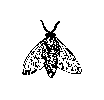
\epsfig{file=fly.eps, height=1in, width=1in}
% \caption{A sample black and white graphic (.eps format)
% that has been resized with the \texttt{epsfig} command.}
% \end{figure}


% As was the case with tables, you may want a figure
% that spans two columns.  To do this, and still to
% ensure proper ``floating'' placement of tables, use the environment
% \textbf{figure*} to enclose the figure and its caption.
% and don't forget to end the environment with
% {figure*}, not {figure}!

% \begin{figure*}
% \centering
% 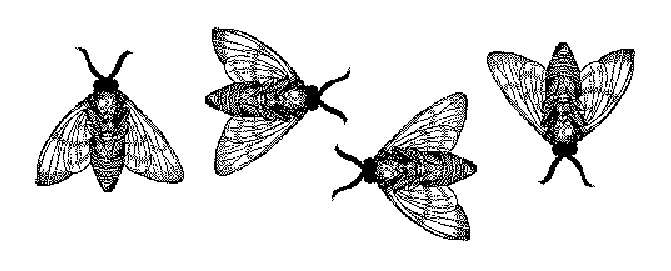
\epsfig{file=flies.eps}
% \caption{A sample black and white graphic (.eps format)
% that needs to span two columns of text.}
% \end{figure*}

% Note that either {\textbf{.ps}} or {\textbf{.eps}} formats are
% used; use
% the \texttt{{\char'134}epsfig} or \texttt{{\char'134}psfig}
% commands as appropriate for the different file types.

% \begin{figure}
% \centering
% % 
\psfig{file=rosette.ps, height=1in, width=1in,}
% \caption{A sample black and white graphic (.ps format) that has
% been resized with the \texttt{psfig} command.}
% \vskip -6pt
% \end{figure}

% \subsection{Theorem-like Constructs}
% Other common constructs that may occur in your article are
% the forms for logical constructs like theorems, axioms,
% corollaries and proofs.  There are
% two forms, one produced by the
% command \texttt{{\char'134}newtheorem} and the
% other by the command \texttt{{\char'134}newdef}; perhaps
% the clearest and easiest way to distinguish them is
% to compare the two in the output of this sample document:

% This uses the \textbf{theorem} environment, created by
% the\linebreak\texttt{{\char'134}newtheorem} command:
% \newtheorem{theorem}{Theorem}
% \begin{theorem}
% Let $f$ be continuous on $[a,b]$.  If $G$ is
% an antiderivative for $f$ on $[a,b]$, then
% \begin{displaymath}\int^b_af(t)dt = G(b) - G(a).\end{displaymath}
% \end{theorem}

% The other uses the \textbf{definition} environment, created
% by the \texttt{{\char'134}newdef} command:
% \newdef{definition}{Definition}
% \begin{definition}
% If $z$ is irrational, then by $e^z$ we mean the
% unique number which has
% logarithm $z$: \begin{displaymath}{\log e^z = z}\end{displaymath}
% \end{definition}

% Two lists of constructs that use one of these
% forms is given in the
% \textit{Author's  Guidelines}.
 
% There is one other similar construct environment, which is
% already set up
% for you; i.e. you must \textit{not} use
% a \texttt{{\char'134}newdef} command to
% create it: the \textbf{proof} environment.  Here
% is a example of its use:
% \begin{proof}
% Suppose on the contrary there exists a real number $L$ such that
% \begin{displaymath}
% \lim_{x\rightarrow\infty} \frac{f(x)}{g(x)} = L.
% \end{displaymath}
% Then
% \begin{displaymath}
% l=\lim_{x\rightarrow c} f(x)
% = \lim_{x\rightarrow c}
% \left[ g{x} \cdot \frac{f(x)}{g(x)} \right ]
% = \lim_{x\rightarrow c} g(x) \cdot \lim_{x\rightarrow c}
% \frac{f(x)}{g(x)} = 0\cdot L = 0,
% \end{displaymath}
% which contradicts our assumption that $l\neq 0$.
% \end{proof}

% Complete rules about using these environments and using the
% two different creation commands are in the
% \textit{Author's Guide}; please consult it for more
% detailed instructions.  If you need to use another construct,
% not listed therein, which you want to have the same
% formatting as the Theorem
% or the Definition\cite{salas:calculus} shown above,
% use the \texttt{{\char'134}newtheorem} or the
% \texttt{{\char'134}newdef} command,
% respectively, to create it.

% \subsection*{A {\secit Caveat} for the \TeX\ Expert}
% Because you have just been given permission to
% use the \texttt{{\char'134}newdef} command to create a
% new form, you might think you can
% use \TeX's \texttt{{\char'134}def} to create a
% new command: \textit{Please refrain from doing this!}
% Remember that your \LaTeX\ source code is primarily intended
% to create camera-ready copy, but may be converted
% to other forms -- e.g. HTML. If you inadvertently omit
% some or all of the \texttt{{\char'134}def}s recompilation will
% be, to say the least, problematic.

% \section{Conclusions}
% This paragraph will end the body of this sample document.
% Remember that you might still have Acknowledgments or
% Appendices; brief samples of these
% follow.  There is still the Bibliography to deal with; and
% we will make a disclaimer about that here: with the exception
% of the reference to the \LaTeX\ book, the citations in
% this paper are to articles which have nothing to
% do with the present subject and are used as
% examples only.

\nocite{*} % Arrian temp

\bibliographystyle{abbrv}
\bibliography{sigproc}  % sigproc.bib
% You must have a proper ".bib" file
%  and remember to run:
% latex bibtex latex latex
% to resolve all references
%
% ACM needs 'a single self-contained file'!


%line 391%
\end{document}
